\subsection{Carbon Black yield and morphology}
The CB volume fraction, $f_v$, and primary particle diameter, $d_p$, characterize the yield and morphology of CB generated during methane pyrolysis, respectively. $f_v$ was determined from the measured extinction at 633nm and 1064nm, considering the reported variability of $E(m)$ in the literature, ranging from 0.174~\citep{lee1981optical} to 0.37~\citep{agafonov2011soot} for 633nm and from 0.2 to 0.46 for 1064nm~\cite{bladh2011optical}. Primary particle diameter, $d_p$, was obtained by visually identifying the primary particles in the TEM images and calculating the arithmetic mean. A minimum of 200 primary particles were measured for each condition, except for $T_5$=1875~K, in which the structure of particles appears as a compact carbonaceous lump rather than a chain-like aggregate, with poorly defined boundaries between primary particles (Fig.~\ref{fig:tem1875}).

The model was optimized by identifying the values of $\eta_{inc}$, $\eta_{ads}$, $\eta_{haca}$, $A_{carb}$, and $E_{carb}$ that minimize the prediction error for both $f_v$ and $d_p$. The optimization assumes that $d_p$  its final value before the end of the process under all conditions, allowing the $d_p$ measured from TEM images to represent the simulation results sampled at 5~ms.


As shown in Fig.~\ref{fig:fv_timehis_comp}a, the optimized model reproduces the time evolution of the measured $f_v$ at 1984~K and 2203~K. The $f_v$ measured by 633~nm is overall larger than that of 1064~nm, which be explained by the contribution of PAHs to absorption at 633~nm~\citep{zerbs2009influence}. The predicted $f_v$ profile exhibits four distinct stages: (i) an initial induction period with negligible CB formation due to low precursors concentrations. The duration of this CB-free stage decreases with temperature, shifting CB inception to earlier times e.g., from approximately 2.3~ms at 1984~K to 0.8~ms at 2203~K using a threshold of 0.01~ppm. (ii) A gradual rise in $f_v$ driven primarily by PAH adsorption (e.g., from 2.3~ms to 3~ms at 1984~K), followed by (iii) an accelerated increase associated due to activation of surface growth via the HACA, e.g., from 3~ms to 4.2~ms at 1984~K. Finally, surface growth slows down as carbonization limits reactive sites, resulting in a nearly constant CB mass. The late-time decline in $f_v = V_{CB}/V_{gas}$ is attributed to gas-phase expansion caused by the arrival of the expansion wave at the endwall, reducing pressure and increasing $V_{gas}$ while $V_{CB}$ remains constant.

As shown in Fig.~\ref{fig:fv_timehis_comp}b, the time evolution of the primary particle diameter, $d_p$, follows the similar trend as $f_v$. The largest $d_p$ is observed at $\mathrm{T_5}=2203$~K, consistent with its highest $f_v$. For all conditions, $d_p$ attains approximately 95\% of its final value by 4.5~ms, indicating the completion of surface growth, since $d_p$ increases only through this mechanism. This observation supports the assumption that TEM images collected well after the test can reliably represent the $d_p$ at the end of 5~ms.

Fig.~\ref{fig:fv_sampled_comp} compares the predicted $f_v$ with measurements at 633~nm and 1064~nm at 2, 3, 4, and 5~ms. The largest $f_v$ occurs at $\mathrm{T_5}$=2203~K, consistent with the peak in A2R5 mole fraction at the same temperature (Fig.~\ref{fig:interm_sampled_comp}), which enhances inception and PAH adsorption rates. For all sampling times, the temperature dependence of $f_v$ follows a bell-shaped profile, consistent with previous observations in the literature~\citep{agafonov2016unified}. At $\mathrm{T_5}$=1875 and 1984~K, the model predictions align more closely with the 1064~nm measurements across all times. In contrast, at $\mathrm{T_5}$=2132, 2203, and 2247~K, the predictions shift closer to the 633~nm data. At the highest temperature, $\mathrm{T_5}$=2355~K, the model underpredicts $f_v$ compared to both wavelengths at all sampling times. The particle mass analysis performed on simulation results (Fig.~\ref{fig:carbon_cont}) indicates accounts for the smallest fraction of soot carbon at all temperatures ($\le2$\%). PAH adsorption is the primary contributor at 1875~K and 1984~K, but its contribution decreases at higher temperatures, where HACA is dominant provides 87\% of CB mass at 2355~K. This is mainly due to to increase in $\mathrm{C_2H_2}$ concentration with temperature (Fig.~\ref{fig:interm_sampled_comp}c) that results in larger HACA rates.

\begin{figure}[!t]
	\centering
	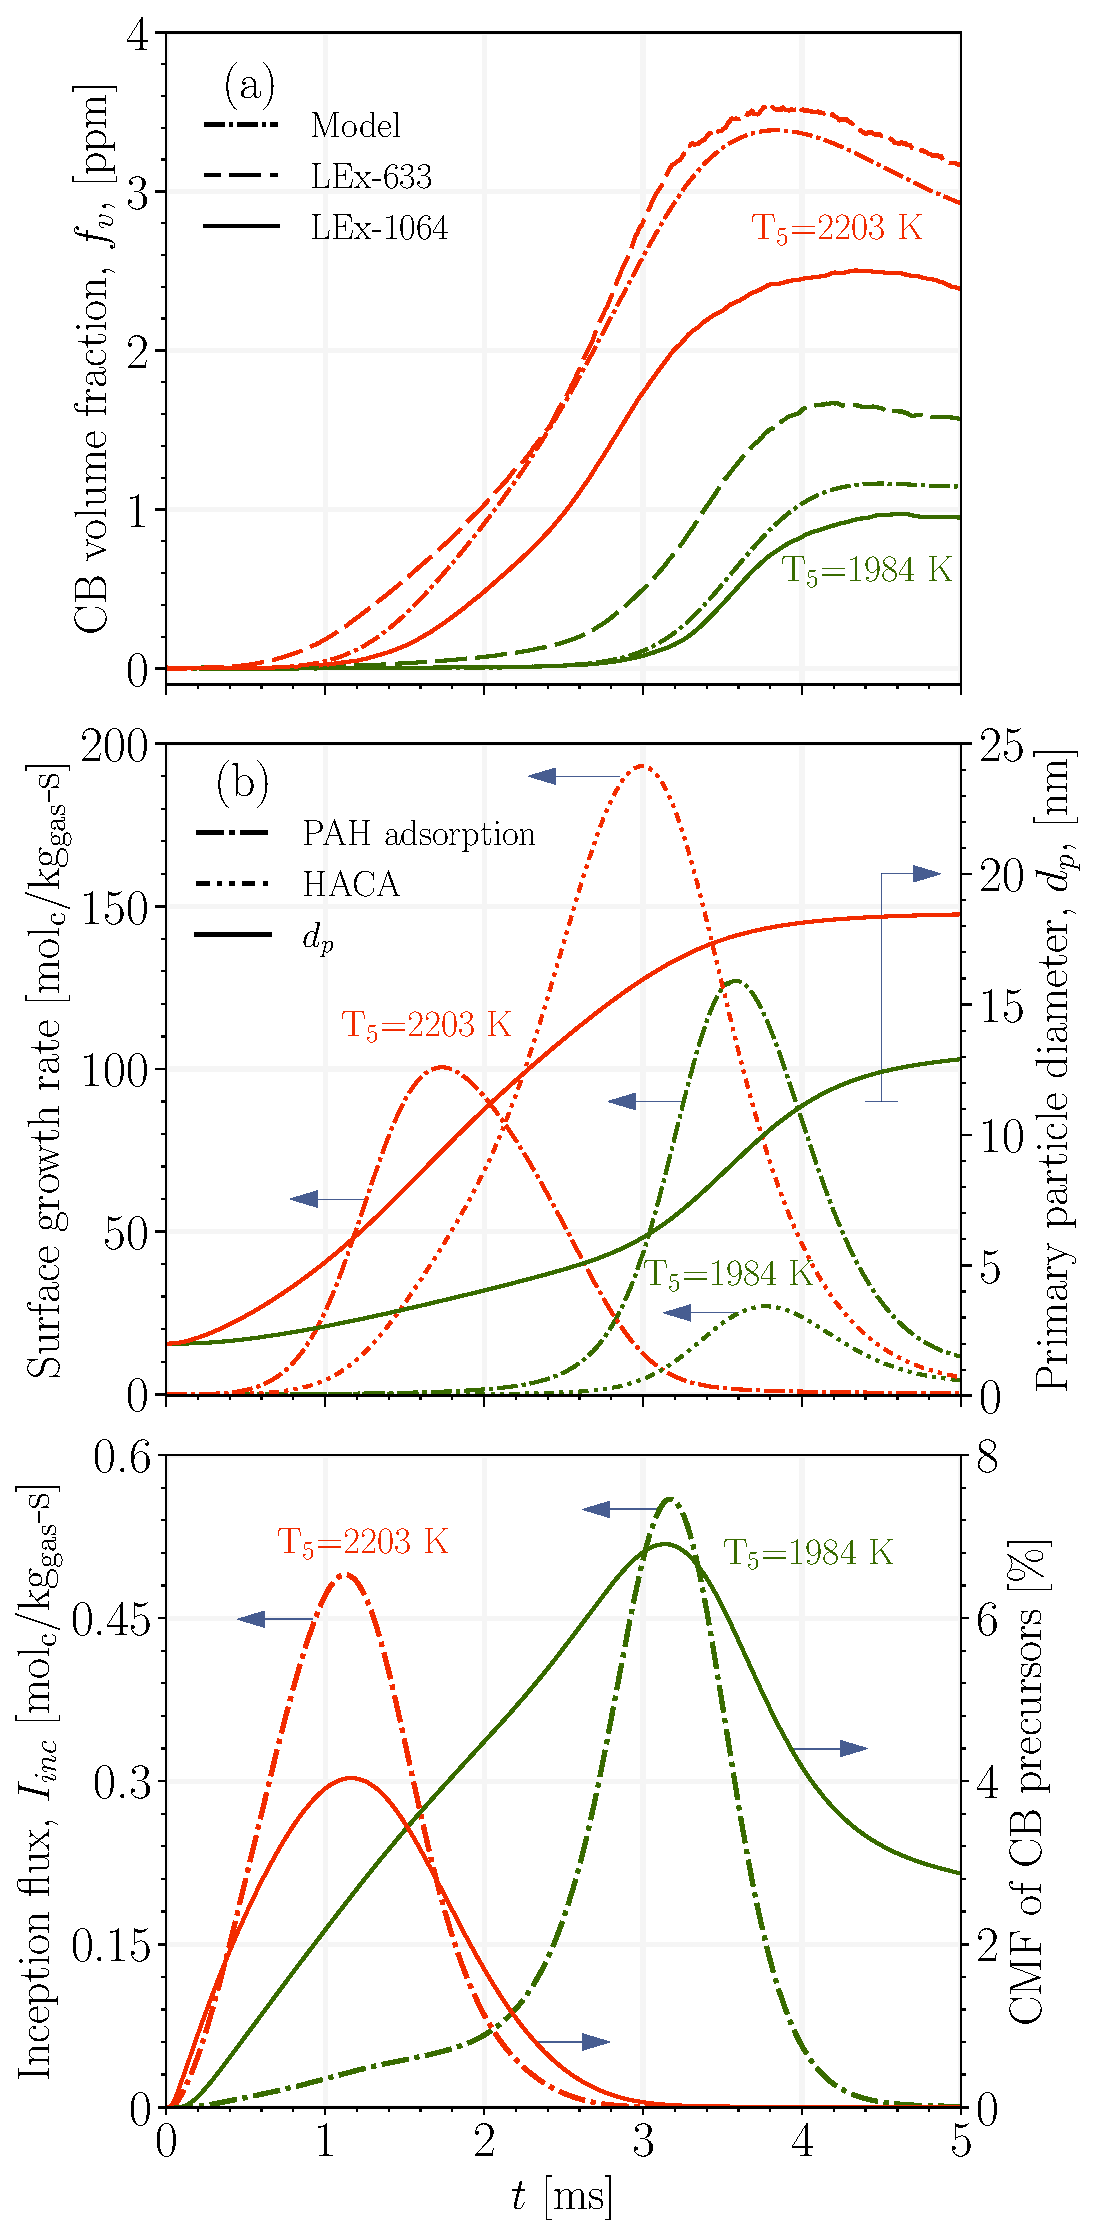
\includegraphics[width=0.3\textwidth]{Figures/time_fv_dp_gr_inc.pdf}
	\caption{The measured time-histories of CB volume fraction, $f_v$ from extinction at 633~nm and 1064~nm (a) compared with the model predictions. The surface growth rate by HACA and PAH adsorption and the primary particle diameter, $d_p$ (b). The uncertainty range of $f_v$ is omitted for clarity.}
	\label{fig:fv_timehis_comp} 
\end{figure}


\begin{figure*}[!t]
	\centering
	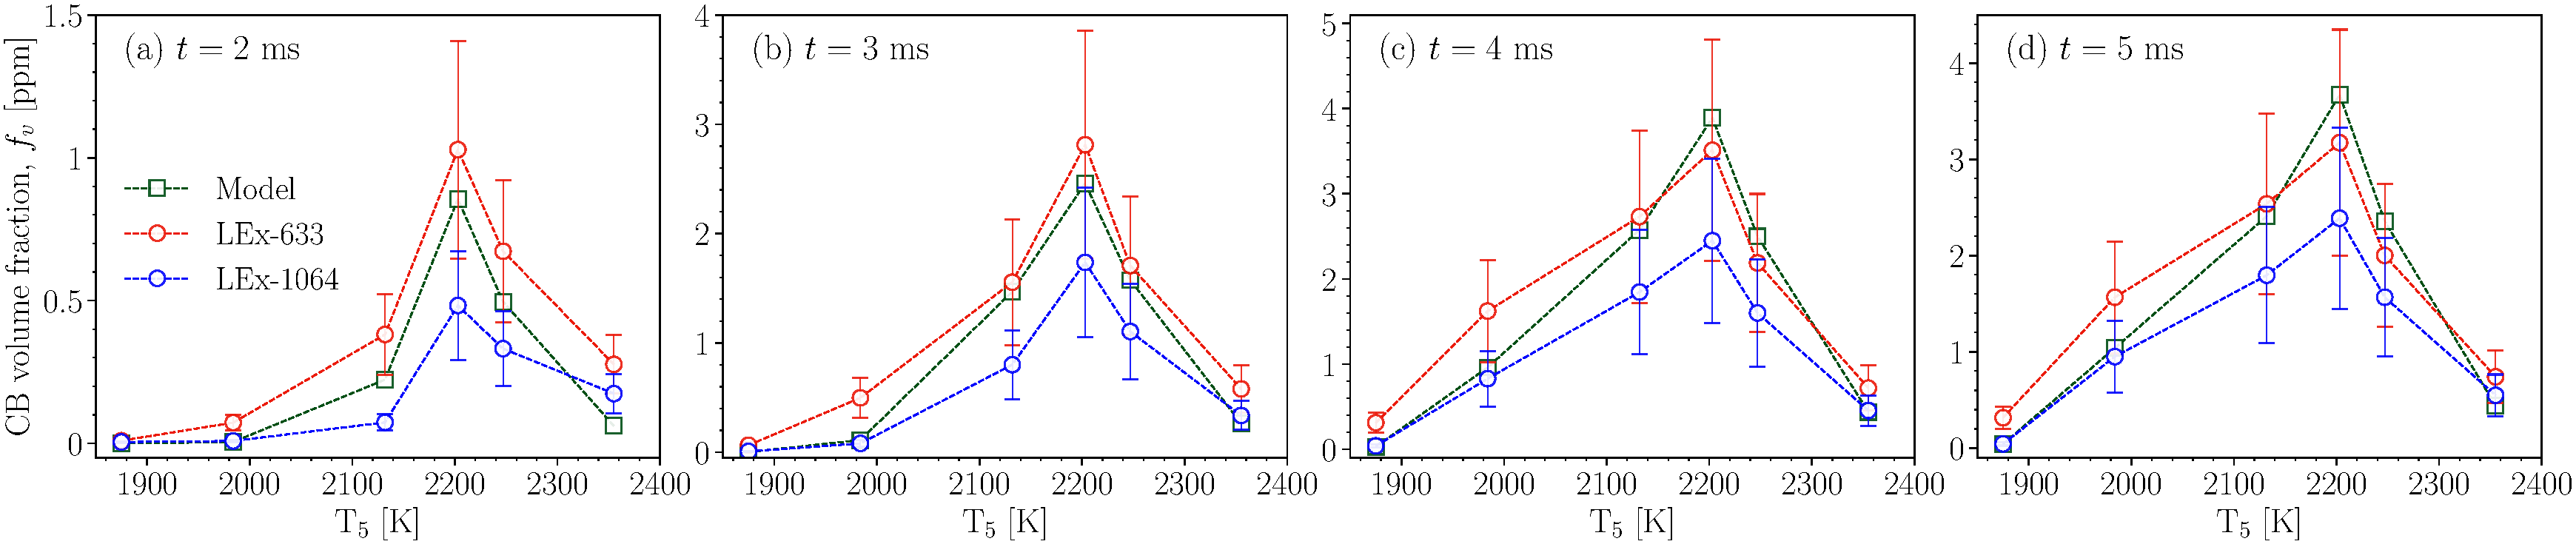
\includegraphics[width=1\textwidth]{Figures/fv_allconds_sampled.pdf}
	\caption{The CB volume fraction, $f_v$, from light extinction at $\lambda=633$~nm sampled at 2~ms (a), 3~ms (b), 4~ms (c), and 5~ms and compared with the simulation results for $\mathrm{T_5}=1875$, 1984, 2132, 2203, 2247, 2355~K. Errors bars indicate experimental uncertainty due to variability in $E(m)$, and the dashed line is added to show the trends.}
	\label{fig:fv_sampled_comp} 
\end{figure*}

As shown in Fig.~\ref{fig:dp_sampled_comp}, $d_p$ obtained from TEM measurements steadily decreases with temperature, while the model predicts an increase up to 2203~K and a decline afterwards, similar to the trend of $f_v$ (Fig.~\ref{fig:fv_sampled_comp}). It can be seen in 

\begin{figure}[!t]
	\centering
	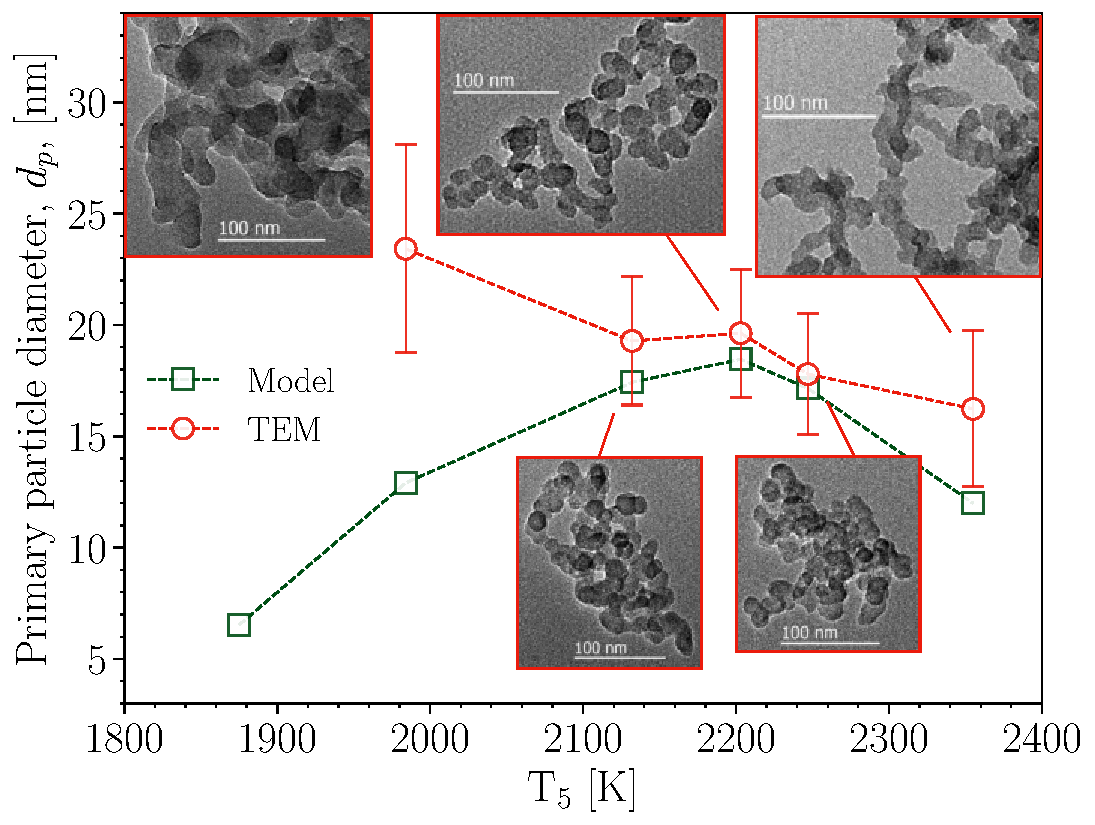
\includegraphics[width=0.48\textwidth]{Figures/dp_allconds_sampled.pdf}
	\caption{The predicted primary particle diameter, $d_p$, at 5~ms compared with the data from the TEM data for $\mathrm{T_5}=1875$, 1984, 2132, 2203, 2247, 2355~K. Errors bars indicate experimental uncertainty due to variability in $E(m)$, and the dashed line is added to show the trends. The insets show representative TEM images of CB agglomerates of different temperature.}
	\label{fig:dp_sampled_comp} 
\end{figure}


\begin{figure}[!t]
	\centering
	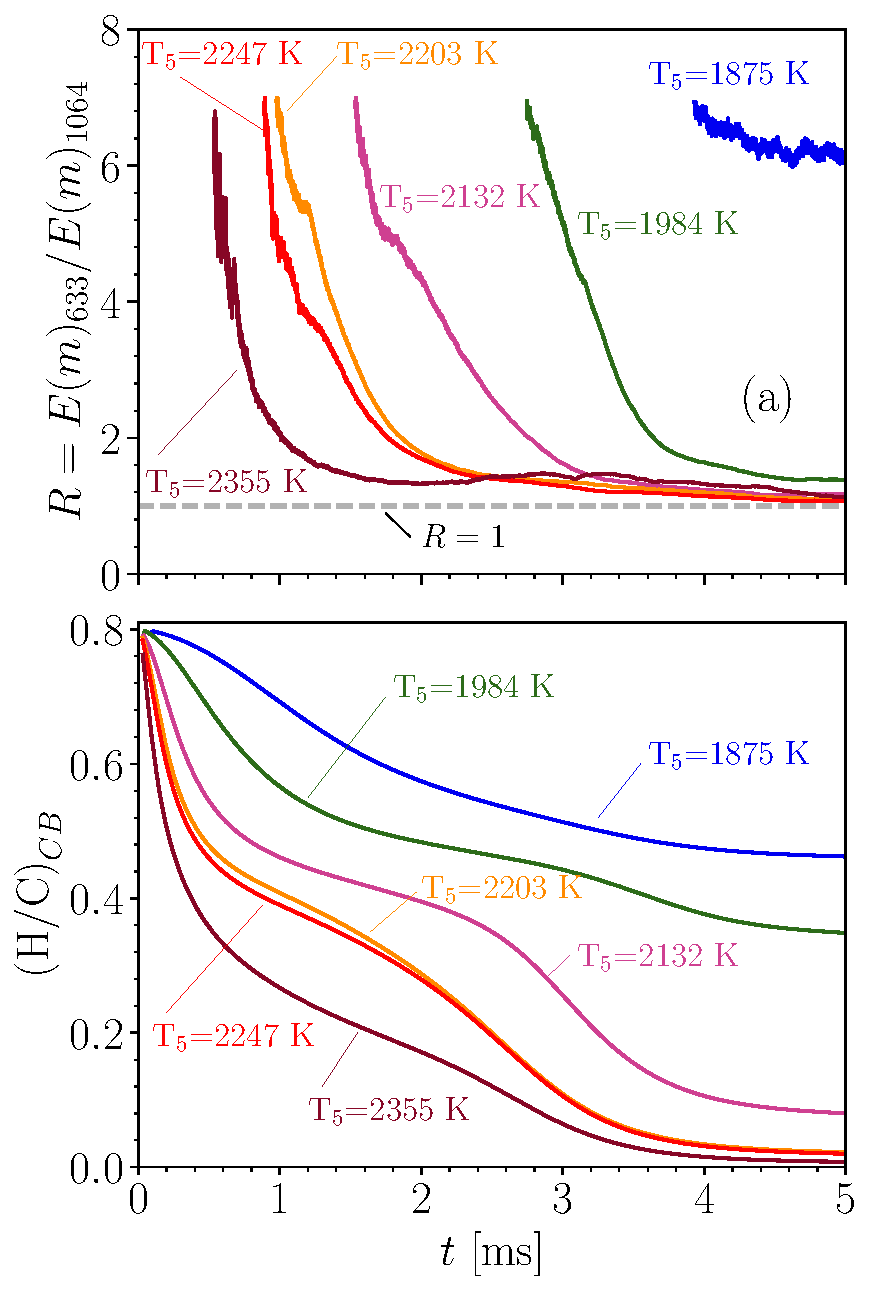
\includegraphics[width=0.38\textwidth]{Figures/htoc_extratio.pdf}
	\caption{The evolution of extinction ratio at 633~nm and 1064~nm, $R=E(m)_{633}/E(m)_{1064}$ from measurements (a), and the predicted H/C ratio of CB particles at $\mathrm{T_5}=1875$, 1984, 2132, 2203, 2247, 2355~K.}
	\label{fig:htoc_extratio} 
\end{figure}